% Compile with XeLaTeX: build.ps1 (Windows) or bash build.sh (Mac/Linux).
\documentclass[12pt,a4paper]{article}
\usepackage{fontspec,polyglossia}
\setdefaultlanguage{russian}
\setotherlanguage{english}
\setmainfont{Times New Roman}
\usepackage{amsmath,amssymb,graphicx,booktabs,float,geometry,setspace}
\usepackage[unicode,hidelinks]{hyperref}
\geometry{left=25mm,right=20mm,top=20mm,bottom=20mm}
\onehalfspacing
\setlength{\parindent}{1.25cm}
\setlength{\emergencystretch}{2em}
\graphicspath{{figures/}{screenshots/}}
% Generated by lab5.py
\newcommand{\ConstantOne}{0{,}388068}
\newcommand{\ConstantTwo}{0{,}00097825}
\newcommand{\LambdaThirty}{0{,}069834}
\newcommand{\DiffractedCount}{198}
\newcommand{\RingOneCount}{106}
\newcommand{\RingTwoCount}{27}
\newcommand{\RingOneFraction}{0{,}5354}
\newcommand{\RingTwoFraction}{0{,}1364}
\newcommand{\SpeedOneTime}{15{,}8}
\newcommand{\SpeedTwoTime}{31{,}5}
\newcommand{\SlopeTwo}{200{,}44}
\newcommand{\InterceptTwo}{1{,}41}
\newcommand{\RSquaredTwo}{0{,}99994}
\newcommand{\OriginResidualTwo}{0{,}63}
\newcommand{\SlopeThree}{242{,}34}
\newcommand{\InterceptThree}{1{,}69}
\newcommand{\RSquaredThree}{0{,}99994}
\newcommand{\OriginResidualThree}{0{,}74}


\begin{document}
\begin{titlepage}
\begin{center}
\begin{spacing}{1.3}
\textbf{МИНИСТЕРСТВО ОБРАЗОВАНИЯ РЕСПУБЛИКИ БЕЛАРУСЬ}\\[0.25cm]
\textbf{БЕЛОРУССКИЙ ГОСУДАРСТВЕННЫЙ УНИВЕРСИТЕТ}\\[0.25cm]
\textbf{ФАКУЛЬТЕТ МЕХАНИКО-МАТЕМАТИЧЕСКИЙ}\\[0.25cm]
\textbf{Кафедра веб-технологий и компьютерного моделирования}
\end{spacing}
\vspace{4.2cm}
\textbf{ВОЛНЫ ДЕ БРОЙЛЯ И ДИФРАКЦИЯ ЭЛЕКТРОНОВ}\\[0.4cm]
Лабораторная работа № 5
\end{center}
\vspace{3.6cm}
\noindent\hspace*{0.48\textwidth}\begin{minipage}{0.52\textwidth}
\begin{spacing}{1.0}
Панасика Владислава Александровича\\
обучающегося 4 курса специальности\\
«Математика и компьютерные науки»\\[0.6cm]
Научный руководитель:\\
ассистент КФОиПИ,\\
Полякова Яна Владимировна
\end{spacing}
\end{minipage}
\vfill
\begin{center}Минск, 2026\end{center}
\end{titlepage}
\setcounter{page}{2}
\tableofcontents
\clearpage

\section{Цель работы и расчётные формулы}
Цель --- исследовать статистический характер дифракции электронов,
зависимость радиусов колец от ускоряющего напряжения и определить
межплоскостные расстояния и индексы Миллера железа.
Электронограммы и исходная статистика получены в предоставленном
виртуальном электронографе difraction.exe; выбран образец железа.
Сохранены снимки окон и электронограмм при масштабе $\times4$.

По заданию $L=757$ мм, $a=2{,}87$ \AA{},
$h=6{,}63\cdot10^{-34}$ Дж$\cdot$с,
$m=0{,}911\cdot10^{-30}$ кг,
$e=1{,}602\cdot10^{-19}$ Кл, $c=2{,}998\cdot10^8$ м/с.
Длина волны де Бройля с релятивистской поправкой:
\begin{equation}
 \lambda=\frac hp=
 \frac{h}{\sqrt{2meV\left(1+\frac{eV}{2mc^2}\right)}}
 =\frac{C_1}{\sqrt{V_{\mathrm{кВ}}(1+C_2V_{\mathrm{кВ}})}}.
\end{equation}
Здесь при $\lambda$ в \AA{} и $V$ в кВ:
$C_1=\ConstantOne$ \AA$\cdot$кВ$^{1/2}$,
$C_2=\ConstantTwo$ кВ$^{-1}$.

Условие Вульфа--Брэгга и геометрия электронограммы:
\begin{equation}
 2d\sin\theta=n\lambda,\qquad
 R=L\tan(2\theta)\approx\frac{nL\lambda}{d},\qquad
 d\approx\frac{nL\lambda}{R}.
\end{equation}
Угол рассеяния равен $2\theta$. Для кубической решётки
\begin{equation}
 d=\frac a{\sqrt{h^2+k^2+l^2}},\qquad
 S=\left(\frac ad\right)^2=h^2+k^2+l^2.
\end{equation}

Радиусы считывались по положениям колец на сохранённых изображениях.
Цена малого деления линейки --- 1 мм; при $\times4$ масштаб снимков
составляет около 5,43 пикселя/мм. Радиусы приведены до 0,1 мм,
характерная точность отсчёта оценивается порядком 0,2 мм.
Накопление тёмных пикселей использовано только для нахождения положения
колец; число электронов взято из таблицы программы.
Расчёт таблиц и построение графиков по отсчётам выполнены в Python.

\clearpage
\section{Упражнение 1. Статистический характер дифракции}
При 40, 60 и 120 кВ получены электронограммы для 10, 1000 и
10\,000 выпущенных электронов. Все изображения имеют одинаковый масштаб.
\begin{figure}[H]
\centering
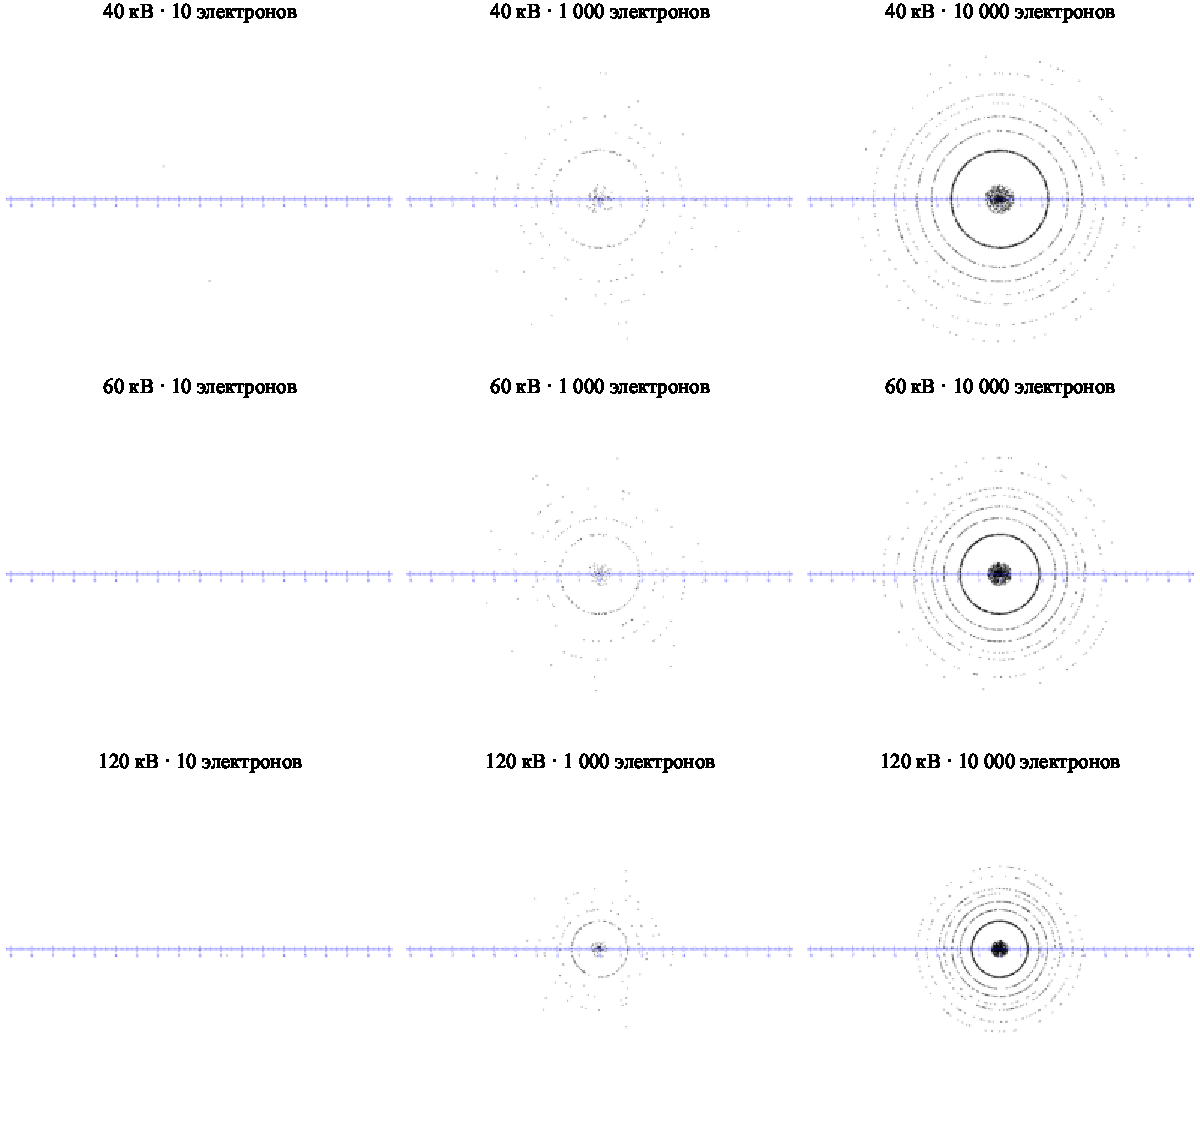
\includegraphics[width=0.95\textwidth]{task1_accumulation.pdf}
\caption{Снимки электронограмм из виртуального электронографа.
Строки: 40, 60, 120 кВ; столбцы: 10, 1000, 10\,000 электронов.}
\end{figure}
При малом числе электронов видны отдельные точки, при накоплении ---
дифракционные кольца. С ростом напряжения импульс увеличивается,
длина волны уменьшается, поэтому кольца сжимаются.

\clearpage
\subsection{Влияние темпа вылета и исходная статистика}
При 40 кВ выполнены два пуска по 1000 электронов с различным темпом.
Длительность составила около \SpeedOneTime{} и \SpeedTwoTime{} с.
Положения колец сохраняются; изменяются время накопления и случайное
расположение отдельных меток. Это согласуется с независимым прохождением
электронов: для дифракции не требуется взаимодействие разных электронов.
\begin{figure}[H]
\centering
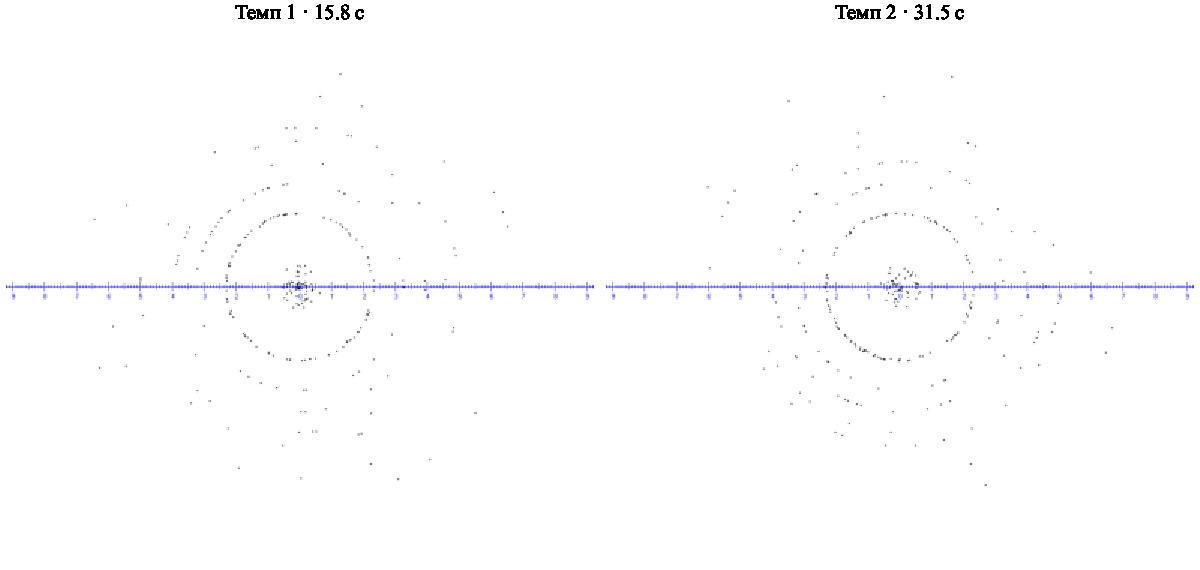
\includegraphics[width=0.92\textwidth]{task1_speeds.pdf}
\caption{Две серии при одинаковых напряжении и числе электронов,
но разных темпах вылета.}
\end{figure}

Для статистического исследования выполнен отдельный пуск:
40 кВ, $k_0=1000$, шаг 50. Встроенный график программы показывает
$k_1/k_0$, $k_3/k_0$ и $k_4/k_0$.
\begin{figure}[H]
\centering
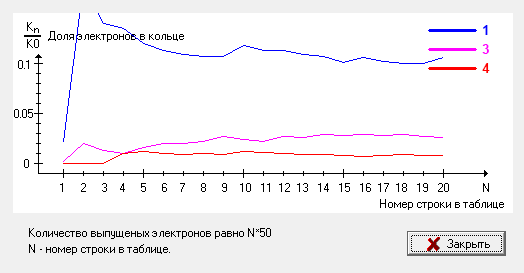
\includegraphics[width=0.78\textwidth]{task1_statistics_graph.png}
\caption{Исходный снимок статистического графика программы.}
\end{figure}
По условию требуются доли $k_j/k$, где $k$ --- число попаданий во все
семь колец. Поэтому для первых двух колец выполнен пересчёт
по экранной таблице распределения.

\clearpage
\subsection{Доли попаданий и их вероятностный смысл}
Использованы обозначения
\begin{equation}
 k=k_1+\cdots+k_7,\qquad f_j=\frac{k_j}{k}.
\end{equation}
Центральный пучок не включён в $k$. Из таблицы программы перенесены
20 строк значений $k_1/k_0$, $k_2/k_0$ и $k$; по ним восстановлены
целые $k_1,k_2$ и рассчитаны требуемые доли.
\begin{figure}[H]
\centering
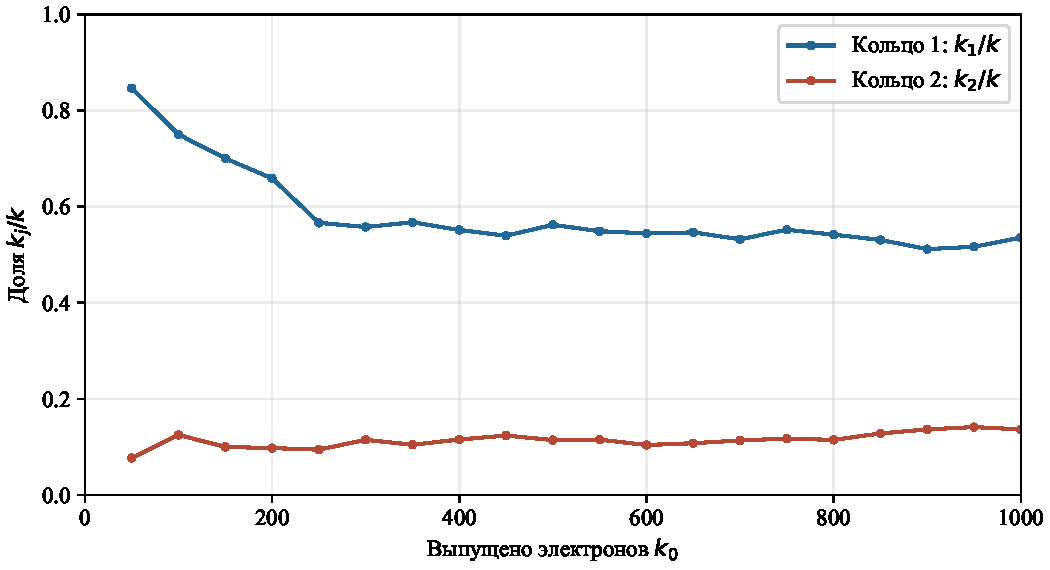
\includegraphics[width=0.96\textwidth]{task1_statistics.pdf}
\caption{Доли попаданий в первое и второе кольца среди всех
дифрагированных электронов; данные таблицы виртуального опыта.}
\end{figure}
В конце серии $k=\DiffractedCount$, $k_1=\RingOneCount$,
$k_2=\RingTwoCount$. Следовательно,
\[
 f_1=\frac{\RingOneCount}{\DiffractedCount}=\RingOneFraction,
 \qquad f_2=\frac{\RingTwoCount}{\DiffractedCount}=\RingTwoFraction.
\]
При малом числе событий доли сильно флуктуируют; при накоплении
их колебания обычно уменьшаются. По закону больших чисел частоты
приближаются к вероятностям, но сходимость не обязана быть монотонной.
Для независимых событий характерный разброс доли имеет порядок
\begin{equation}
 \sigma(f_j\mid k)=\sqrt{\frac{q_j(1-q_j)}{k}},
\end{equation}
где $q_j$ --- вероятность попадания в кольцо при условии попадания
в одно из колец. Отдельный электрон даёт точку; распределение множества
точек выявляет волновую закономерность.

\clearpage
\section{Упражнение 2. Зависимость радиусов от напряжения}
Для 30, 37, 47, 61, 83 и 120 кВ получены серии по 20\,000 электронов.
Измерены радиусы второго и третьего колец. Рассчитана величина
\begin{equation}
 X=\frac1{\sqrt{V(1+C_2V)}}.
\end{equation}
При постоянных $d,n,L$ из теории следует $R=nLC_1X/d$ --- прямая
через начало координат.
\begin{table}[H]
\centering
\caption{Отсчёты по электронограммам и расчёт длины волны}
\begin{tabular}{rrrrr}
\toprule
$V$, кВ & $\lambda$, \AA & $X$, кВ$^{-1/2}$ & $R_2$, мм & $R_3$, мм\\
\midrule
\input results/voltage_rows.tex
\bottomrule
\end{tabular}
\end{table}
\begin{figure}[H]
\centering
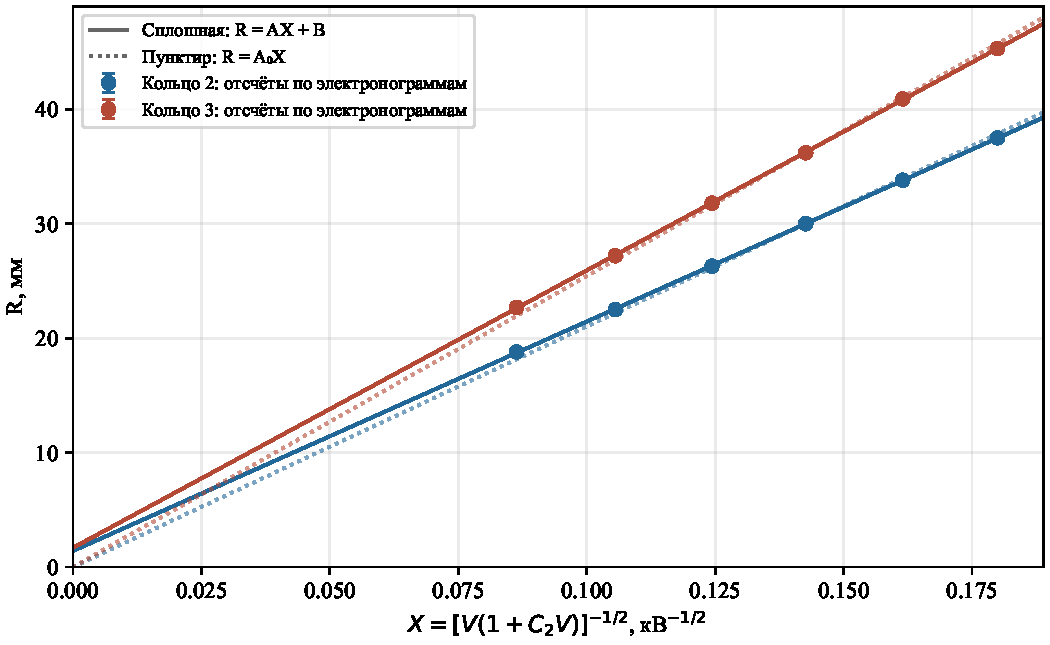
\includegraphics[width=0.89\textwidth]{task2_voltage.pdf}
\caption{Радиусы колец в зависимости от $X$.
Сплошные линии --- МНК с $R=AX+B$, пунктирные --- с $B=0$.
Вертикальные отрезки показывают ориентир отсчёта 0,2 мм.}
\end{figure}
Аппроксимации дали $R_2=\SlopeTwo X+\InterceptTwo$ и
$R_3=\SlopeThree X+\InterceptThree$;
$R^2=\RSquaredTwo$ и $\RSquaredThree$ соответственно.

\clearpage
\subsection{Электронограммы и вывод о соотношении де Бройля}
\begin{figure}[H]
\centering
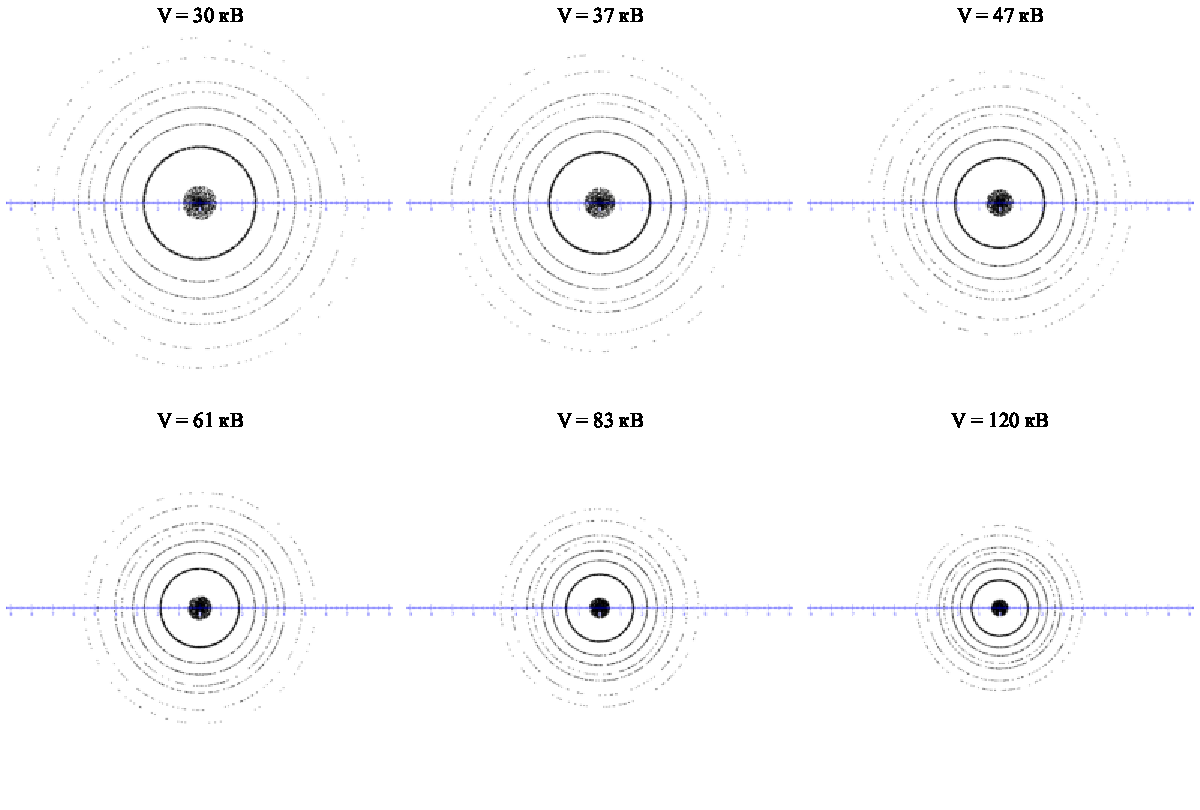
\includegraphics[width=0.98\textwidth]{task2_electronograms.pdf}
\caption{Исходные электронограммы при шести напряжениях;
масштаб $\times4$, по 20\,000 электронов.}
\end{figure}
Радиусы уменьшаются с ростом напряжения, что качественно согласуется
с соотношением де Бройля. Зависимости $R(X)$ близки к прямым, однако
свободные члены не равны нулю. При принудительном $B=0$ максимальные
остатки составляют \OriginResidualTwo{} и \OriginResidualThree{} мм,
что превышает ориентир отсчёта 0,2 мм.

Положения колец в предоставленном приложении масштабируются
приближённо как $V^{-1/2}$. Поэтому полученные виртуальные данные
воспроизводят общий тренд, но не дают точного подтверждения
релятивистской поправки. Высокое $R^2$ само по себе не подтверждает
требуемое прохождение прямой через начало координат.

\clearpage
\section{Упражнение 3. Межплоскостные расстояния и индексы}
При 30 кВ получена электронограмма из 30\,000 электронов;
$\lambda=\LambdaThirty$ \AA. Измерены радиусы первых пяти колец.
\begin{figure}[H]
\centering
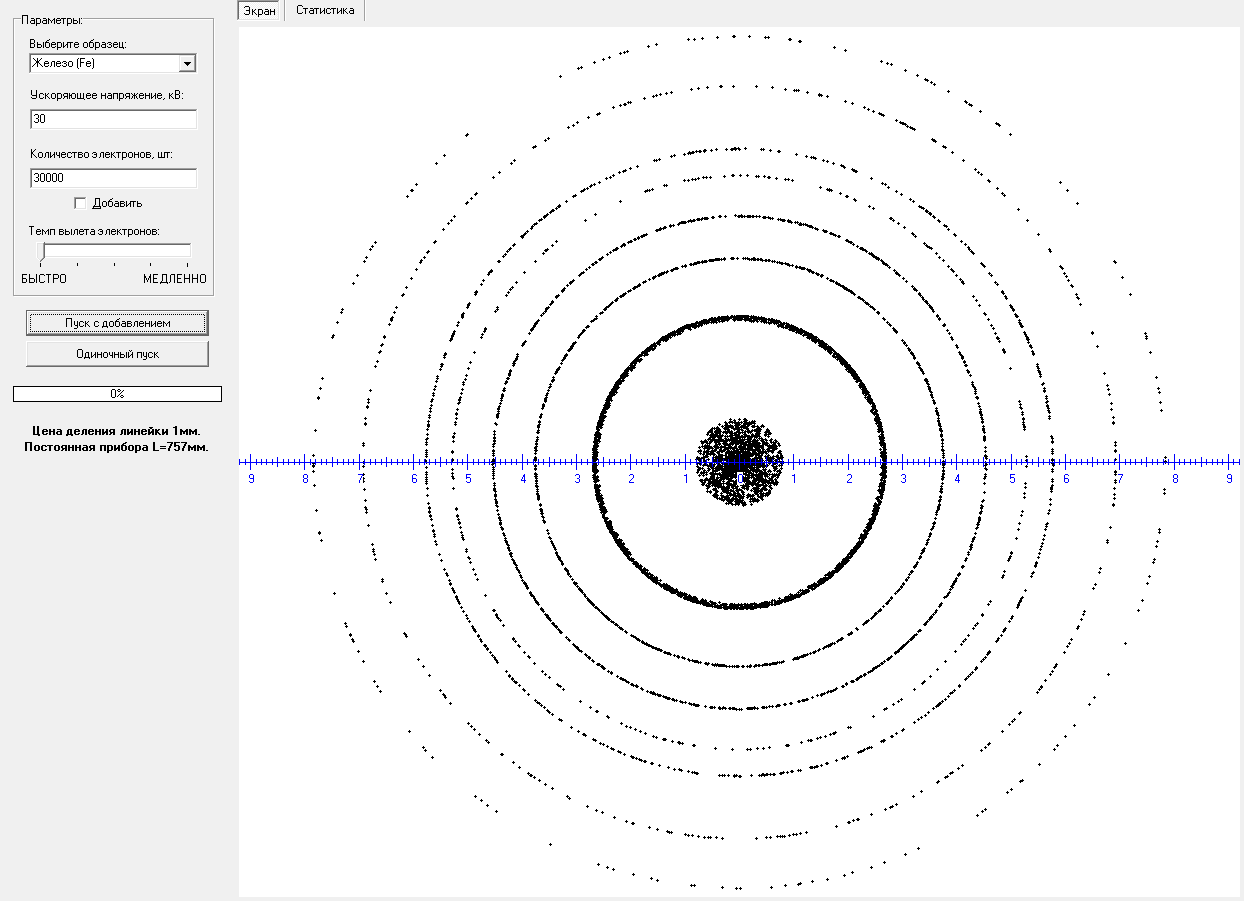
\includegraphics[width=0.91\textwidth]{task3_30kV_30000_window.png}
\caption{Снимок окна электронографа: железо, 30 кВ, 30\,000 электронов.}
\end{figure}
Вычислены $d=nL\lambda/R$ и $S=(a/d)^2$.
Для кольца №4 принят $n=2$, для остальных $n=1$.
\begin{table}[H]
\centering
\caption{Межплоскостные расстояния и индексы Миллера}
\begin{tabular}{rrrrrrr}
\toprule
№ & $n$ & $R$, мм & $d$, \AA & $S$ & $[S]$ & $(hkl)$\\
\midrule
\input results/structure_rows.tex
\bottomrule
\end{tabular}
\end{table}
После округления $S$ подобраны целые $h,k,l$.
Для ОЦК-железа сумма $h+k+l$ чётная. Четвёртое кольцо соответствует
$(110)$ во втором порядке, эквивалентному $(220)$ в первом порядке.

Такой анализ дифракционных колец используют для определения
кристаллических фаз и исследования структуры тонких образцов.
\end{document}
